\chapter{Measurements}
In \refsec{prototype} we consolidated our goals for a tool like COOP. One of those goals was for it to improve the performance of a target program and never worsen it. In this chapter we will discuss COOP's results and see that the outcomes of our optimization varies greatly and depend on the target program. We will also see that COOP (while working as intended on some) is by nature not a generic fit for any kind of program, as its optimization potential derives from the target program's structure and access patterns.\\
Further there are a few different traits we want to measure about COOP. The optimization effects; Different heuristics on field weight evaluations; COOP's run times.

\section{COOP's impact on performance}
In order to see the affects of our optimization on a target program, we will measure its run-time and its frames per second (if something like a 'game-loop' is given).\\
Cache utilization will be tested with \textit{Valgrind}'s dedicated tool \textit{Cachegrind} created by Nicholas Nethercote. Valgrind runs programs on a simulated CPU. When specifically regarding improvements in cache friendliness this saves us from external factors like other processes thrashing our cache-lines. This way we can run isolated tests to compare the un-/optimized versions of our target program. In case of Cachegrind it will explicitly simulate a cache hierarchy and observe e.g. accesses and misses for us. Cachegrind is an amazing tool, since it is easy to use, works out of the box and is completely free.

\subsection{Low complexity test scenario}
To quickly see where the strengths and weaknesses of COOP are we will first observe the results of a very simple test case. This is the quickest way to see possible improvements/deteriorations and the easiest way to reason about how certain aspects impact certain numbers. For our first simple test we will define an arbitrary struct, its fields and some access patterns, that should enable COOP to refine the cache utilization. Lets just go with our NPC from the previous chapters.
\begin{lstlisting}[language=C++, name={Simple test code in order to make first tests. It will heavily use an NPC's positional properties (pos, vel) and basically disregard the fields name, age and mood, as they would be accessed based on user generated events.}, label={simple_test}]
struct NPC {
	float pos[3];
	char * const name; //unfavorable structure padding!
	float vel[3];
	int age, mood;
	[some constructors]
};

int main(){
	//classic OOP initializations
	NPC **npcs = new NPC*[N];
	for(unsigned i = 0; i < N; ++i)
	{
		npcs[i] = new NPC([ini arguments]);
	}
	
	//some positional-domain calculations
	for(unsigned i = 0; i < N; ++i)
	{
		some_calculation(npcs[i].pos, npcs[i].vel, delta_time);
	}	
	[event based data accesses to other/cold fields]
	[cleanup code]
}
\end{lstlisting}
After running COOP on this code we will identify the fields \textit{name, age} and \textit{mood} as cold fields. We build both the optimized and the unoptimized versions several times gradually increasing \textit{N} in order to demonstrate how COOP behaves on growing data capacities. In the following graphs we will oppose the optimized- and the unoptimized versions where \textit{(ac)} marks the values \textit{\textbf{a}fter \textbf{c}oop} has been applied, so the 'optimized' values.
\begin{figure}[ht]
	\begin{minipage}[b]{0.333\linewidth}
		\centering
		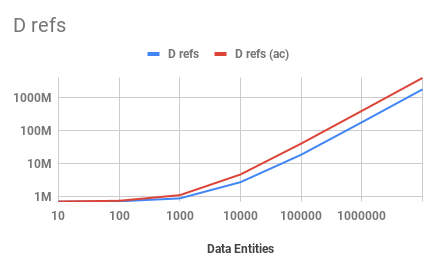
\includegraphics[width=\textwidth,height=\textwidth]{PICs/test_file_d_refs}
	\end{minipage}
\hspace{-0.3cm}
	\begin{minipage}[b]{0.333\linewidth}
		\centering
		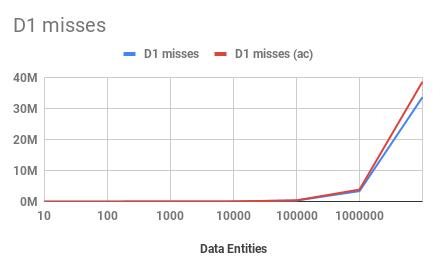
\includegraphics[width=\textwidth,height=\textwidth]{PICs/test_file_d1_misses}
	\end{minipage}
\hspace{-0.3cm}
	\begin{minipage}[b]{0.333\linewidth}
		\centering
		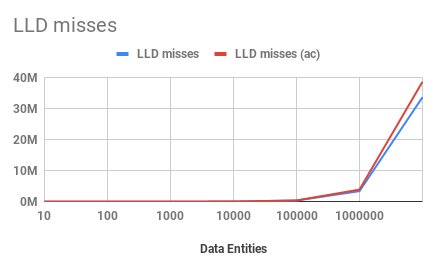
\includegraphics[width=\textwidth,height=\textwidth]{PICs/test_file_lld_misses}
	\end{minipage}
\vspace{-0.5cm}
\caption{Measurements for \textit{N} data entities and the resulting cache utilizations. The red line marks the 'post-optimization' values. Note that the \textit{D refs} graph uses a logarithmic scale so the increase in D refs as N grows actually becomes very large!}
\label{test_file_is_it_bad}
\end{figure}
When looking at the number of cache misses \reffig{test_file_is_it_bad} reveals alarming numbers. Despite our optimization, that specifically is designed to reduce cache misses we not only somehow managed to increase the amount of cache misses, but also the number of total data accesses! At this point COOP looks bad and further looking at the execution times we will see, that there is actually an observable deterioration in run time as well \reffigp{test_file_execution_times}.
\begin{figure}[!htbp]
	\centering
	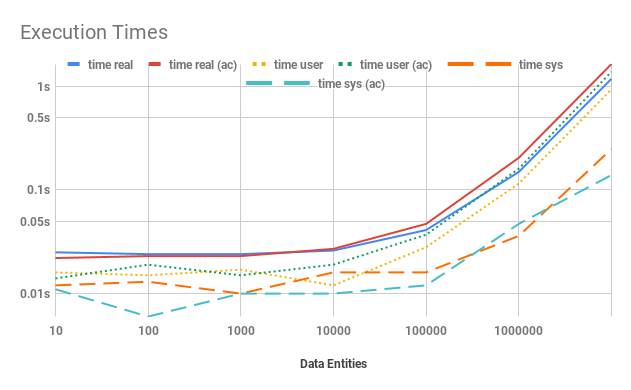
\includegraphics[width=0.85\textwidth, height=0.5\textwidth]{PICs/test_file_execution_times}
	\caption{Measured runtimes for un-/optimized versions of our simple test code with rising N. These measurements have been made by using the Unix command \textit{time}.}
	\label{test_file_execution_times}
\end{figure}
While moving time spent away from the operating system by interchanging heap allocations with placement news to our bss data works well in the beginning, the overhead of initializing our free list grows linearly with the amount of data. While the operating system's free list that will handle our heap allocations already exists on a user program start, our custom allocator introduces additional overhead to the program, that will ultimately pitch towards inferior initialization overhead that might outscale the benefits of its fast allocation times.\\
Our specialized memory solution also is responsible for the additional data accesses, as well as the additional cache misses. Cachegrind offers post processing tools as well, like \textit{cg\_annotate}, that provides a per function statistic on cache misses etc. As we initialize the two free lists (one for the hot and one for the cold data) we will also produce cache misses scaling linearly with our \textit{N}.\\\\
In our particular case not only our custom memory management adds initialization overhead, but it also won't improve the data layouts situation. The whole point of our pool allocator was for the single heap allocations to be contiguous in memory. In this particular test case, the data entities are sequentially allocated on the heap. Those allocations are made on a fresh heap, so even though this initialization pattern is prone to heap fragmentation in this case there is no prior fragmentation. Also since the entities will only be deallocated on program end, hence no new allocations during computation and possible fragmentation overhead, our pool allocator will effectively have no positive impact on the program. 
\begin{figure}[!htbp]
	\centering
	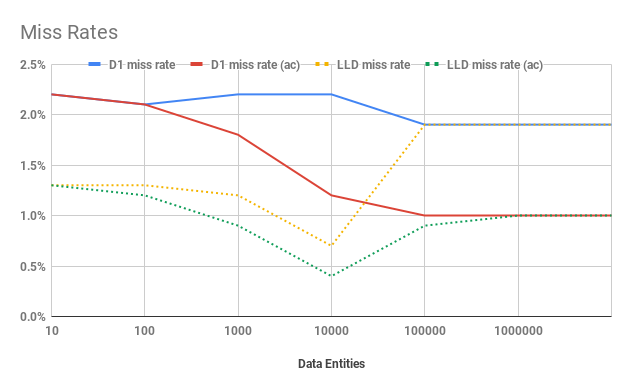
\includegraphics[width=0.85\textwidth, height=0.5\textwidth]{PICs/test_file_miss_rates}
	\caption{The small test programs miss rates show improvement, as the cold data no longer resides unused in our cache. Note how the last level cache miss rates rise between 10,000 and 100,000 entities due to the total amount of our data exceeding the cache size.}
	\label{test_file_miss_rates}
\end{figure}
What about cache utilization? Even though increased initialization overhead adds yet more cache misses, shouldn't we at least have improved the access on the data during computation?\\
\reffig{test_file_miss_rates} illustrates the miss rates of our test programs with growing \textit{N}. We can observe, that the unoptimized versions of our test program have higher miss rates even though there are more data accesses in general. As the data in both the optimized and unoptimized versions is contiguous in memory, this is solely attributable to the difference in the data layout produced by our optimization.\\\\
While our affect on the data layout was beneficial, the assumption, that single heap allocation initializations are inherently bad depends on the target programs complexity and data flow. Further static analysis could potentially identify bad initialization patterns more precisely but more on that in TODO REF SEC FUTURE WORK AND PROBLEMS.

\subsection{Testing an OOP particle system}
Our next test will work with a more complex target project, a particle system. While it will be deliberately programmed in a rather OOP manner and completely managed by the CPU, it will also provide us with an example of a program with undetermined runtime as there will be a 'game loop' and the user will trigger the program stop. In this case we would measure the targets delta times or FPS(frames per second), to see whether or not COOP can induce an improvement.\\
Specifically we will create a scene with four particle systems each shooting a bunch of particles at a center point, so the particles from the different systems collide and bounce off each other. The systems load will increase with several parameters: The particles life time; The particle systems fire rate; the size of the bulks that are released at once. All those factors affect the total amount of particles that will be in the scene at one discrete time step.\\\\
Besides the rendering there will be one other significant part to the program. The physics. The computation of all the collisions and resulting changes to velocities, accelerations and ultimately positions will demand most of the CPUs resources and will happen once per frame. When increasing the total amount of particles in the scene, we will experience higher delta times, as processing their individual state changes will consume more and more time. Besides observing our optimization's impact on the cache utilization we will compare the programs' delta times over a fixed amount of frames \reffigp{delta_times}.\\
The particles' setup is a rather simple POD (plain old data) type with all the data we need, for example a particles position, acceleration, velocity, mass, lifetime, radius, texture and shader. COOP's static analysis will yield field weightings as can be seen in \reffig{particle_field_weights}.
\begin{figure}[!htbp]
	\centering
	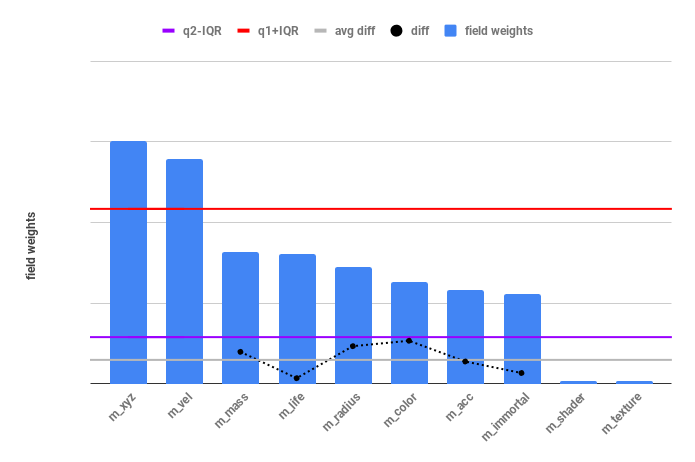
\includegraphics[width=0.7\textwidth,height=0.5\textwidth]{PICs/particle_field_weights}
	\caption{The particle's field weighst according to COOP. The q1/2 are the quartiles, that together with the interquartile range define our spike points. Inside the mid fragment we will induce further significance grouping as discussed in \refsec{sig_groups}.}
	\label{particle_field_weights}
\end{figure}
The shader and texture fields were determined to be relatively cold enough to favor a split. This seems strange, as they will be used each frame, however our heuristic assumes, that hiving them off will benefit the other fields' computations enough to achieve improved cache utilization. In fact in the original version of the test program COOP would state, that it could not detect a favorable split, so it was deliberately worsened. Originally the shader and texture fields were merely pointers to their respective objects. To provoke bad cache utilization we instead let the particle directly hold their instances increasing the overall particles size to a point, where COOP would see optimization potential.\\\\
Now with the shader and texture field externalized to a cold struct the following differences in run time behavior were found \reffig{delta_times}.
\begin{figure}[!htbp]
	\centering
	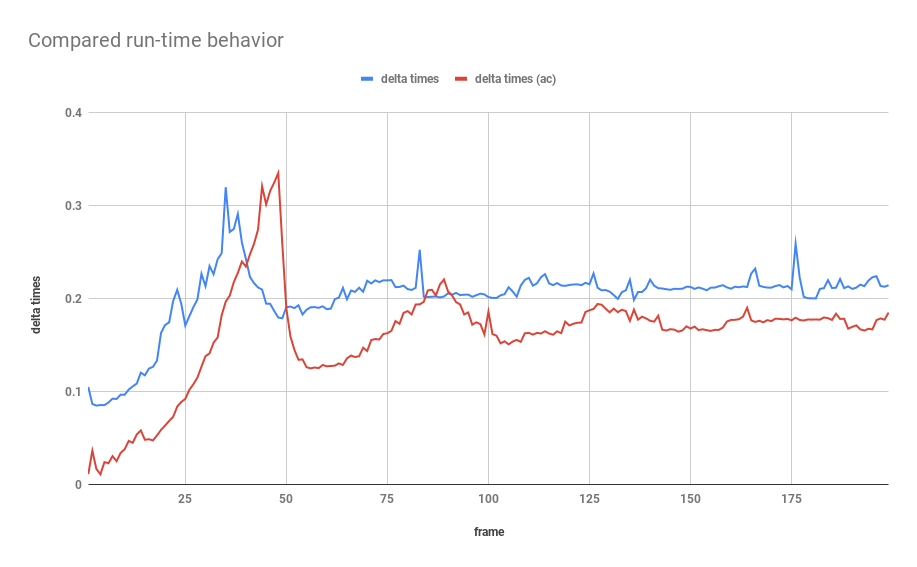
\includegraphics[width=0.8\textwidth,height=0.6\textwidth]{PICs/delta_times}
	\caption{Observed delta times for both the optimized and unoptimized versions of our particle demo. The red line marks the delta times after the optimization was applied and shows that with our less frequently used fields externalized we can accomplish improvement. These measurements were made with approximately 96,000 particles.}
	\label{delta_times}
\end{figure}
Comparing the two builds through cachegrind we find, that COOP successfully reduced the level one data cache's miss rate from 9.5\% to 9.1\% and the last level data cache's miss rate from 0.9\% to 0.7\%.\\\\
How is it, that in this case we could measure improvement when our simple test showed that initial initialization overhead might outscale improved cache utilization? The particles cold data is indeed managed by our pool allocator that is initialized on program start, however we are now measuring frame times inside a game loop. The additional initialization overhead still exists only the applications purpose differs. In this case the trade off is worth, as the initial overhead is comparably insignificant to constant improvement over an undetermined amount of frames.\\\\
Right now this looks promising, given that the target application profits more from an improved data layout than it suffers from program load overhead. However our particle system can easily be used in a way that resembles its actual usage in a real application and the results will be completely different. Lets now introduce a new instance of a particle system to our scene. Additionally to the four particle cannons from before we now initialize a system that will be a nice little fire. Its particles will have a short lifetime starting white gradually turning red and finally turn to black smoke particles. The relevant part however is that those particles won't be colliding with other ones. While COOP right now won't notice that in any way its actual implications for our application are huge.\\
Right now (as said before) the physics steps is a major part of our little demo and those particles won't even bother to run through all those computations. With a colliding/non-colliding particles ratio of only 1:60 we have lost all our previous advantage \reffigp{delta_times_fire}.
\begin{figure}[!htbp]
	\centering
	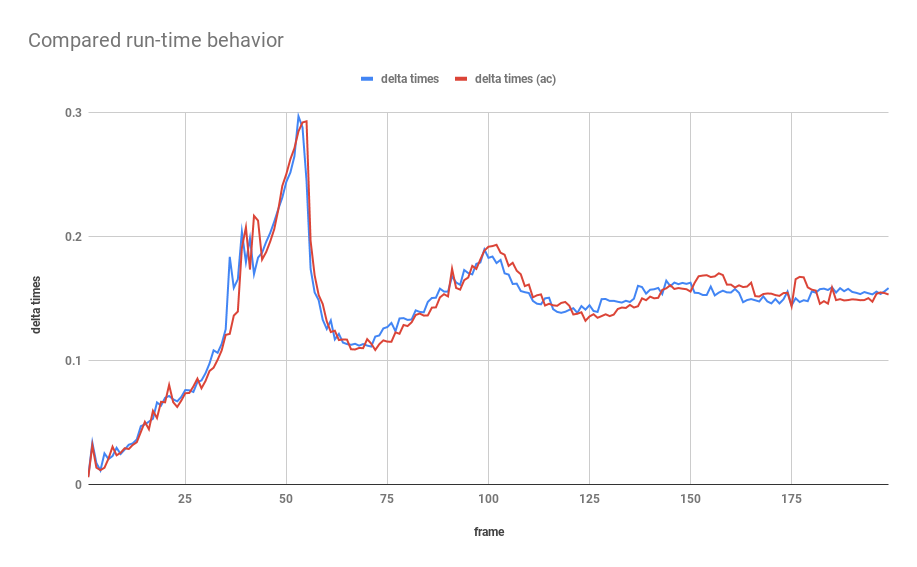
\includegraphics[width=0.8\textwidth,height=0.6\textwidth]{PICs/delta_times_fire}
	\caption{Compared delta times of an optimized and an unoptimized build showing that COOP's metrics have major issues with variant behavior of splitted instances.}
	\label{delta_times_fire}
\end{figure}
We introduced a mere 1000 fire particles to a scene handling up to 60,000 colliding particles. While a thousand particles not having to calculate collision would usually not have a great impact on our system, now it does. Taking away the 'field weights' of other fields like position, velocity, radius and acceleration that are all highly important to physics calculations the externalized fields shader and texture become relatively more significant.\\
While the split is beneficial for one subset of the particles, it is now hazardous for another. With a data capacity that exceeds our cache size this becomes increasingly deteriorating, as more and more cache misses on frequently used data will continuously make slow loads from the lower hierarchy memory units. This is a major issue for COOP and will also be discussed further in TODO REF SEC FUTURE WORK AND PROBLEMS.





